%Dieser Abschnitt beinhaltet die Hintergrundgeschichte (Story) des Spiels. Eine Story ist wichtig für ein Spiel, um zu erklären, warum bestimmte Aktionen durchgeführt werden können, oder nicht. Eine Story ist auch ein einfacher Weg, um eine Umgebung zu schaffen, mit der sich ein Spieler identifizieren kann und Spaß daran hat, die Umgebung zu erforschen und sich darin zu bewegen.

Es ist die wohl älteste Geschichte der Welt. Die Geschichte vom erbitterten
Kampf ums Überleben, den jedes Lebewesen auf dieser Welt Tag für Tag wieder für
sich entscheiden muss. Schon lange wird unser Planet von den verschiedensten
Lebensformen bevölkert, und ebenso lange machen Krankheiten das Leben der
Erdenbewohner gefährlicher und beschwerlicher. Doch gibt es immer wieder
Menschen und Tiere, die manche Krankheiten besser überstehen als andere --
warum das so ist, blieb für lange Zeit im Verborgenen. Heute wissen wir mehr
darüber: Wir wissen von den winzigen Viren und Bakterien, die unermüdlich die
Zellen anderer Lebewesen angreifen, und die Betroffenen haben komplexe Systeme
entwickelt, um sie abzuwehren. Nun liegt es an Ihnen, die richtige Strategie
zum richtigen Zeitpunkt anzuwenden und die Krankheitserreger zurückzudrängen.

\subsection{Konzeptzeichnungen und Prototypen}
\begin{figure}[ht]
  \begin{center}
    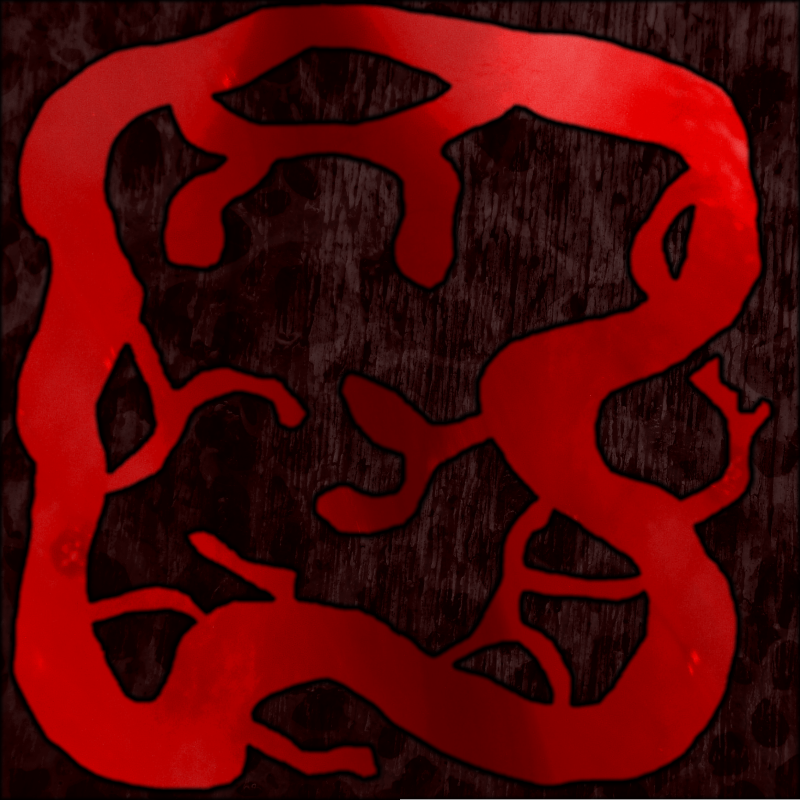
\includegraphics[width=12cm]{./img_screenplay/map_small}
  \end{center}
  \caption{Exemplarischer Aufbau der Karte}
  \label{fig:karte}
\end{figure}

\begin{figure}[ht]
  \begin{center}
    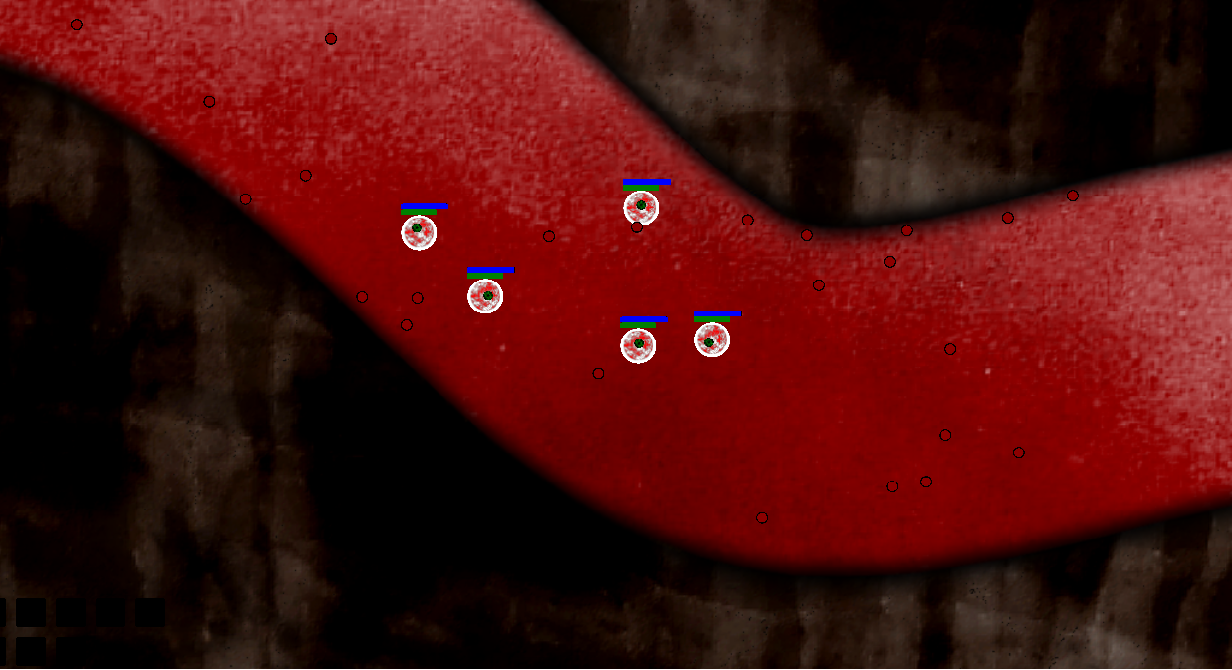
\includegraphics[width=12cm]{img_screenplay/neutral}
  \end{center}
  \caption{Rote Blutkörperchen in einer Blutbahn}
  \label{fig:heamo_virus}
\end{figure}

\begin{figure}[ht]
  \begin{center}
    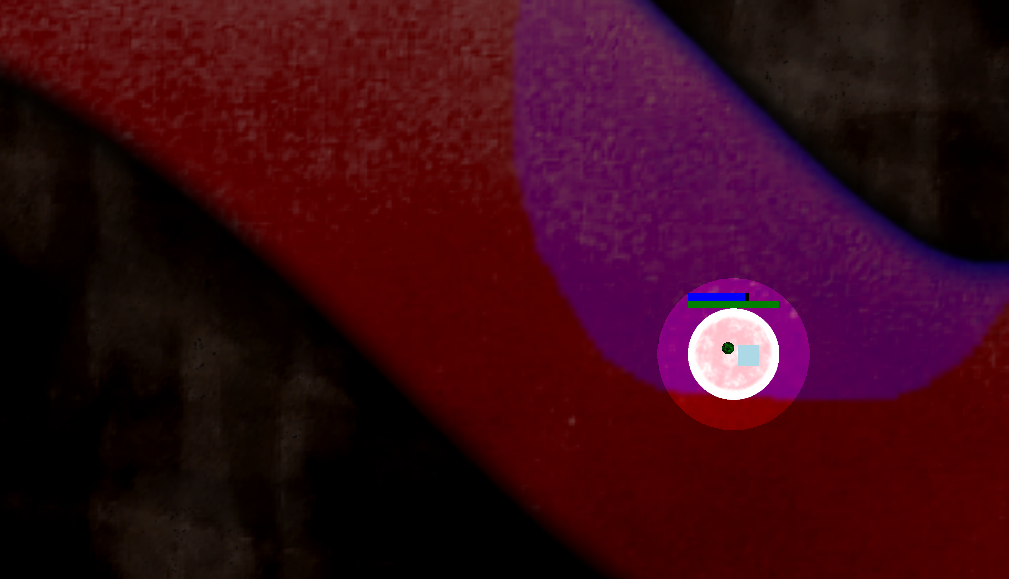
\includegraphics[width=12cm]{img_screenplay/tcell}
  \end{center}
  \caption{T-Zelle im Mutationsfeld}
  \label{fig:tcell}
\end{figure}

\begin{figure}[ht]
  \begin{center}
    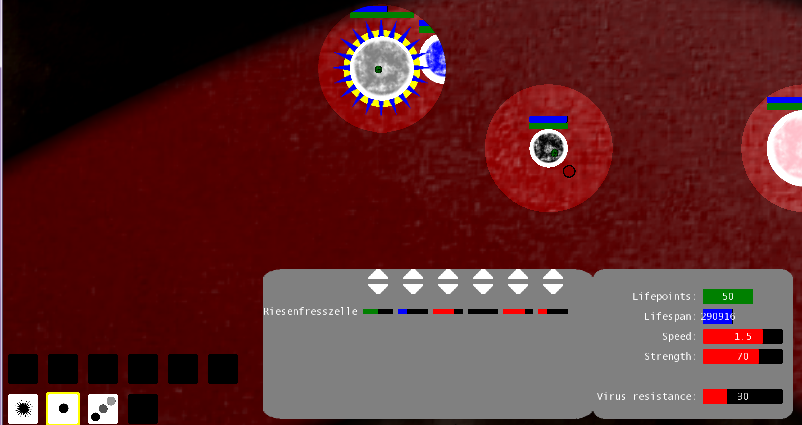
\includegraphics[width=12cm]{img_screenplay/riesenfresszelle}
  \end{center}
  \caption{Riesenfresszelle (grau), mit Sichtradius, die Virus (blau) angreift.
  Prototyp des HUD.}
  \label{fig:macrophage}
\end{figure}


%Konzeptzeichnungen & Storyboards
%Bilder sind wichtig für den ersten Eindruck. Vor allem im GDD sind Konzeptzeichnungen und Skizzen gut aufgehoben. Auf diese Weise kann man nicht nur sich selbst schnell eine Vorstellung von den Ideen machen, sondern auch anderen vermitteln, worum es im Spiel geht und wie das Spiel und seine Geschichte aussieht. 
